\documentclass[titlepage]{article}
\usepackage{ctex}
\usepackage{geometry}
\usepackage{float}
\usepackage{graphicx}
\usepackage{listings}
\usepackage{multirow}
\usepackage{latexsym,bm,amsmath,amssymb}

\begin{document}

\title{Report for Computer System Final Project}
\author{李文昊\quad 王凡\\ 上海交通大学ACM班}
\date{2015.6.17}
\maketitle

\kaishu

\begin{abstract}
\quad \quad 本文记录了我们于2015年的计算机体系结构课程中使用Verilog HDL实现的一个简易Pipeline的相关工作,包括Pipeline的基本架构、
各个阶段、Branch Predictor、Cache、Testbench的实现,用于测试的MIPS Code以及其运行结果分析。
\end{abstract}

\tableofcontents
\newpage

\section{Project概览}
在本课程设计中,我们实现了一个能够处理简单算术运算以及逻辑运算、跳转指令、内存读写操作的基于五级Pipeline架构的处理器(其具体实现见src
目录)。其架构可见下图:
\begin{figure}[H]
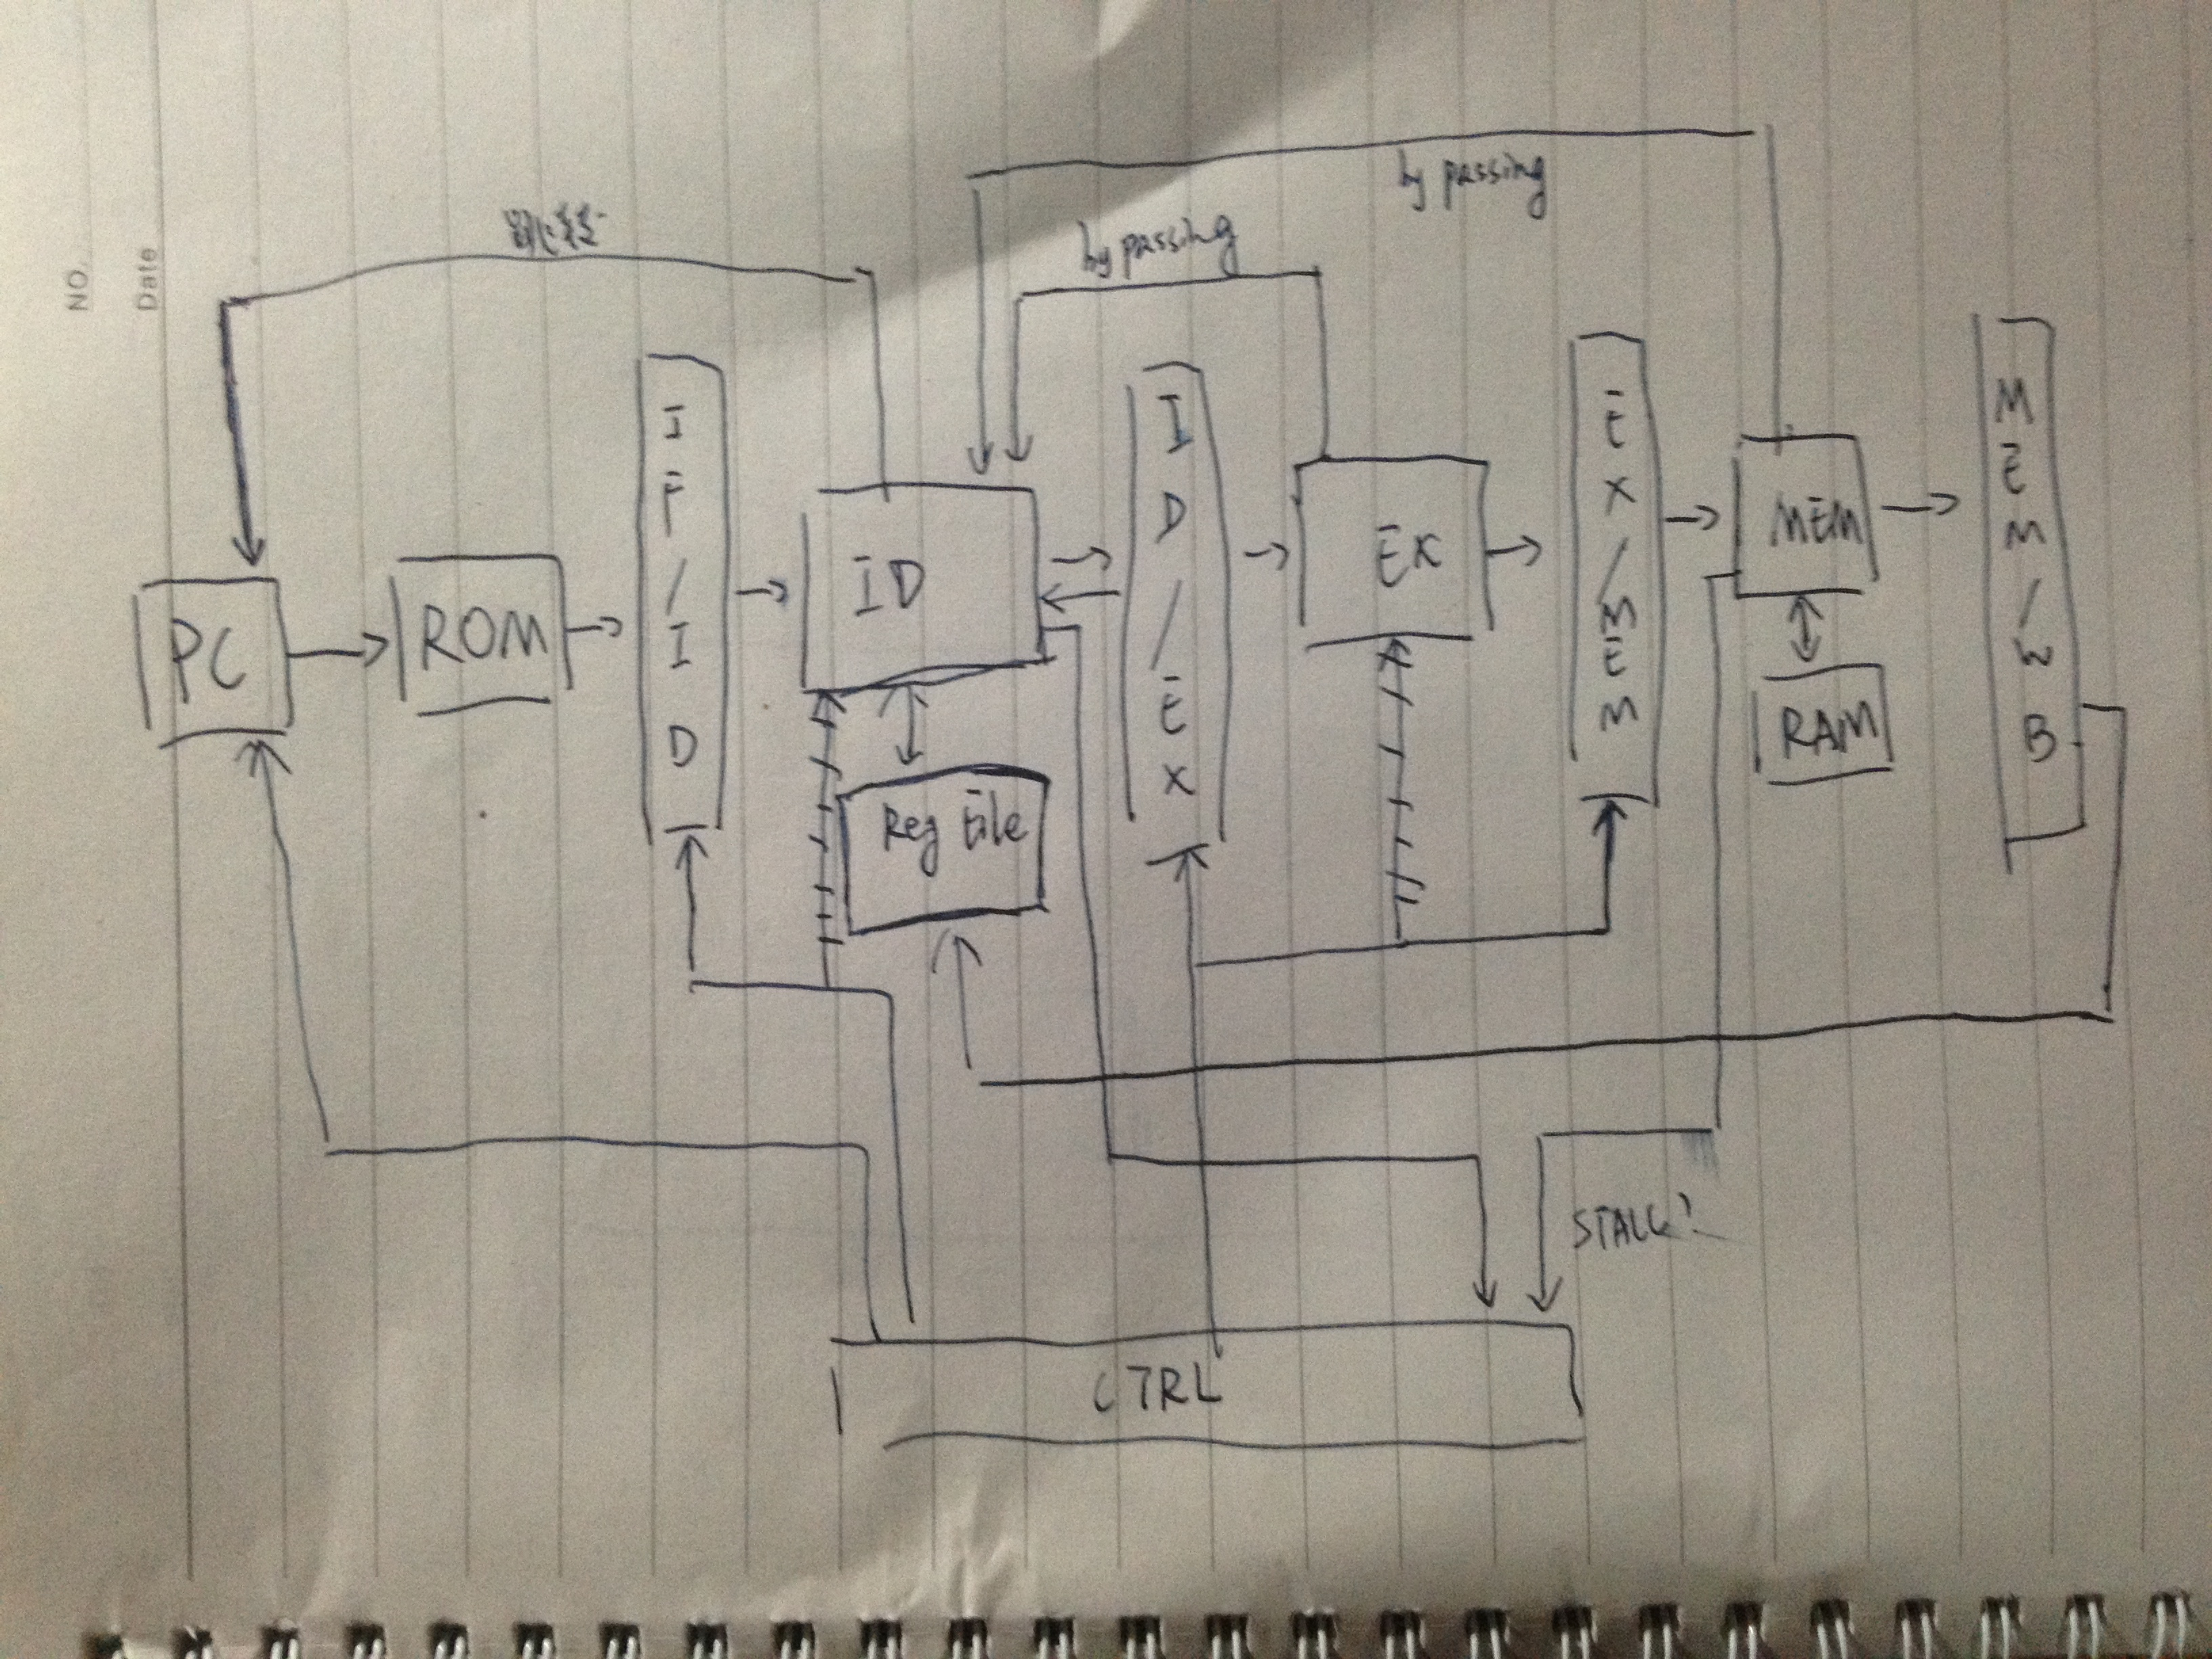
\includegraphics[height=.5\textheight]{constructure.JPG}
\end{figure}
上图中,\emph{ROM}为指令存储器,而\emph{RAM}中包含了内存和缓存。由图可知,我们实现了从\emph{EX}到\emph{ID}、\emph{MEM}到\emph{ID}阶
段的Bypassing,并且支持Pipeline各级的暂停机制,此外我们还实现了一个基于2-bit自动机的Branch Predictor。其连线的实现可见src目录下的
binder.v以及binder\_ram\_rom.v文件,前者连接了五级Pipeline的各基本单元,后者将前者与\emph{ROM}、\emph{RAM}连接。同时我们提供了
testbench文件,见src目录下testbench.v。\\
\indent 接下来各章将分别介绍我们各个阶段的具体实现。
\section{IF阶段}
在每个时钟上升沿,\emph{PC}会向\emph{ROM}提供下一条指令的地址,\emph{ROM}读取相应指令后将其传给\emph{IF/ID},如果不考虑跳转指令,这个
过程每次就是将\emph{PC}中存储的地址加4,非常trivial。然而考虑到跳转指令以及Branch Predictor的实现,就要在此之上新增一些接口以及连线。\\
\indent 我们实现的是一个基于2-bit自动机的Branch Predictor,与老师上课时讲的相同:
\begin{figure}[H]
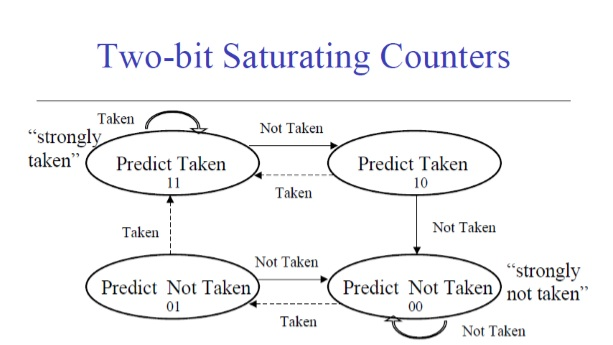
\includegraphics{bp.JPG}
\end{figure}
它实现在\emph{PC}中,初始状态为11。由于是对跳转指令的下一条指令进行Predict,所以\emph{PC}还记录了上一条指令是否是跳转指令,如果是,则根据
当前的自动机状态来决定是否跳转,并将是否跳转作为信息传递到之后的阶段。此外,\emph{ROM}向后不仅传递指令,还传递了指令的地址。这样在\emph{ID}
阶段,通过比较传递来的跳转信息可以知道Predict的正确性,若发生错误则向\emph{PC}传递一个地址,表示应当跳转到的地址,若正确则什么都不做。
当\emph{PC}接收到\emph{ID}传来的地址,则说明上次预测错误了,修改自动机状态。\\
\indent 至此还有一个问题,当预测错误时,预测错的那条指令会进入\emph{IF}阶段,我们要想方法把它kill掉。我们采用的方法是在\emph{ID}阶段打
一个延迟槽标记,记录下一条指令是否在延迟槽中,将其传递给\emph{ID/EX},并在下一个上升沿的时候由\emph{ID/EX}传回\emph{ID},表示当前指令
处于延迟槽。若一个指令处于延迟槽中,则以NOP替换它。
\section{ID与EX阶段}
由于\emph{ID}与\emph{EX}阶段的相似度较高,故放在同一章。\\
\indent \emph{ID}阶段分析了指令类型并读取每条指令中需要用到的寄存器的值,读取寄存器的值时按以下优先级由高到低读取:从\emph{EX}阶段
Bypassing回的值、从\emph{MEM}阶段Bypassing回的值、\emph{Regfile}中的值,或者是一个立即数。同时在\emph{ID}阶段还需要判断上一条指令
是否恰好是LW指令,且该LW指令存放的寄存器当前指令是否需要读取。如果是的话则需要将当前指令暂停一个cycle,否则将出现RAW Hazard。\\
\indent 在\emph{EX}阶段,将进行与\emph{ID}阶段类似的分类讨论,进行算术、逻辑运算的计算,并向\emph{ID}阶段Bypassing。
\section{mem阶段以及Cache}
\emph{MEM}阶段是为了处理存在的load指令或者store指令而存在的,如果当前操作的是这两个指令,我们就可能要对内存进行读写,
否则只是一个数据传递。\\
\indent 为了模拟内存的操作,我们写了一个名叫\emph{RAM}的模块,里面开了大量的register来间接地替代内存。
并且为了方便,在\emph{RAM}中加入了\emph{cache}模块。\\
\indent 对内存的读写是一个很慢的过程,会导致大量的时钟周期浪费,在这种五级pipeline的背景下,我们必须要靠stall来保证数据之间不会有竞争关系。
这种时钟周期的浪费是无法彻底解决的,为了隐藏这种大量的时钟周期的浪费,我们设计了一个\emph{cache}来解决这个问题。\\
\indent 由于考虑到要操作的数字可能非常少,只有100个左右,我们的\emph{cache}就只包含4个Block,每个Block能存储16个32位数字,
并且采用了\emph{Full-Associative}的方法,极大的均衡了空间和查找时间的利用。\\
\indent 因为pipeline中大部分的操作都几乎做到了线性,而很少会有很长的stall产生,而\emph{cache}的每次miss所导致的对内存的直接访问将要消
耗200个时钟周期,而且每次hit或者不hit面对的时间消耗是不一定的。为了方便模拟这种200个时钟周期的消耗而不对\emph{MEM}模块带来一些影响,
我对\emph{cache}单独建立了一个模块,并且专门为其设计了一个状态机,当\emph{cache}没有直接hit,我将要在状态机上执行200个空的时钟周期,
并且在最后时刻把数据取出来。为了取得时序逻辑与组合逻辑上不产生冲突,特别设计了两个接口表示\emph{CACHE}阶段是否真的取得了数字,否则就要在\emph{MEM}阶段中进行stall。\\

\section{暂停机制}
由于在\emph{ID}阶段和\emph{MEM}阶段都要进行一部分的stall才能继续执行下去,而这个stall是可能会牵涉到全部5个stage的。

一般情况下,对于在\emph{ID}中的stall,可能需要停止\emph{PC},\emph{IF},\emph{ID}阶段,而\emph{EX},\emph{MEM},\emph{WB}阶段需要继续执行。

而在\emph{MEM}中的stall,可能需要停止\emph{PC},\emph{IF},\emph{ID},\emph{EX},\emph{MEM},而\emph{RAM}和\emph{WB}阶段需要继续执行。

为了做到这种全局的控制,我们设计了一个模块\emph{CTRL}来解决这种stall的问题。

这个模块完全是由组合逻辑完成,分别对于一些stage发来的stall请求,给各个stage发送是否stall的命令。

由于只有在一些中间模块,比如\emph{EX/MEM},\emph{IF/ID}这些阶段才有时序逻辑,所以其实这些暂停指令只要发到这些模块就行了。

但是在实现的时候我们遇到了一个难点,如果我们简单的当一个模块被stall住的时候,就不往这个模块的后继模块传递信息,那么由于它也因为stall接收不到前一个模块传递过来的信息,导致本应该“停住”的信息丢失了。

针对这一点,我重新设计了一下一个中间模块受到stall命令时的行为。

对于每个中间模块,比如\emph{EX/MEM},当\emph{EX}和\emph{MEM}同时是stall或者\emph{EX}是非stall时,他们应该要无阻碍的继续传递数据,这样才能保证就算被stall住,数据也不会因此而流失。

\section{MIPS Code以及运行结果}
为了测试,我们写了以下MIPS Code(见MIPS.S):
\begin{figure}[H]
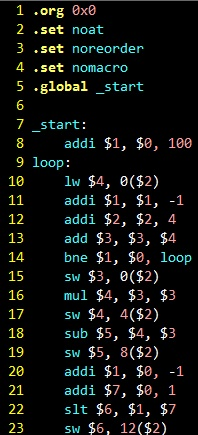
\includegraphics[height=.4\textheight]{mips.JPG}
\end{figure}
它的功能是读入100个数,对其进行求和得$sum$,依次输出$sum$、$sum^2$、$sum^2-sum$、逻辑运算$-1<1$的值。这段代码可以测试基本的算术、逻辑
运算,检查内存读写操作花费的cycle数以及Cache的运作,Branch Predictor是否可以预测while循环的跳转以及Bypassing。我们实现的处理器
经过ModelSim仿真后得到了以下结果(输入的100个数为1到100):
\begin{figure}[H]
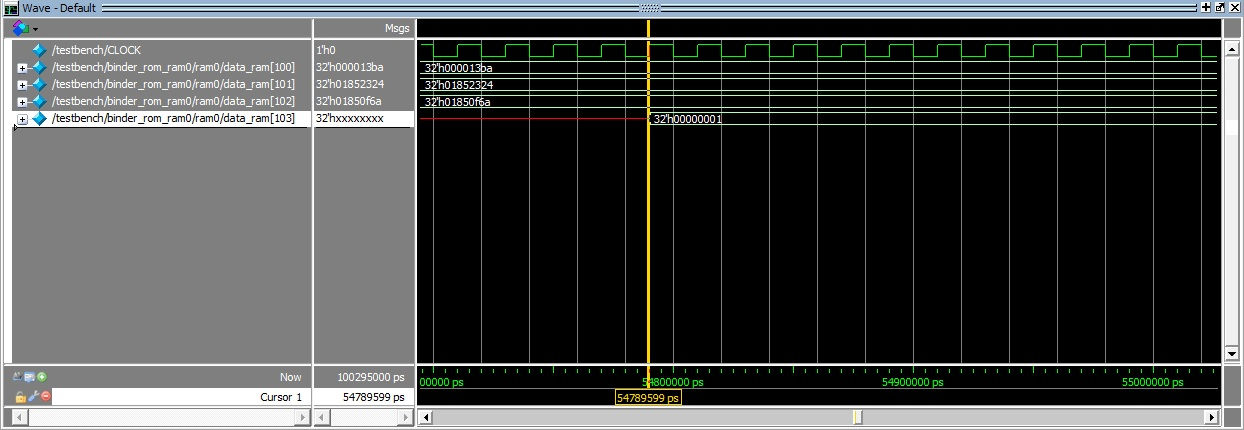
\includegraphics[height=.3\textheight]{1.JPG}
\end{figure}
可以看到,最后写回内存的数(图中为16进制)分别为5050,25502500,25497850和1,是正确的。\\
\indent 我们在testbench中设定20纳秒为一个时钟周期,由图中可见运行完所有的指令花费了约54800纳秒,即约2740个时钟周期。内存读取操作若
Cache Miss则会花费200个周期,内存写固定花费200个周期,在运行之前的MIPS Code时,读取100个数的过程中Cache共Miss了7次,加上之后的4次
写内存操作,共会花费2200个周期。运行该MIPS码时总指令数约为500条,除去内存读写的暂停外共花费了2740-2200约540个时钟周期。经过估算,在不
考虑对内存操作的暂停的情况下,我们的处理器CPI为1。
\section{总结}
虽然整个下来我们并没有实现完备的所有功能,代码量也并没有特别大,但是不得不说这次的Coding对于我们来说是一项挑战,不像平时的编程是建立在一个“算法设计”的思路下,
这次的代码更加是一种“结构设计”,我们需要考虑需要哪些接口,这些接口该怎么连,如何实现停止功能等问题。而且由于组合逻辑和时序逻辑的同时出现,给我们理解整个pipeline运行和
最后的调试带来了极大的困扰。所幸最后还是调试完成了这项工作。

通过这次的project,我们对pipeline的如何运作有了更为深刻的理解。之前在课堂上只是抽象的知道了一些技术,比如branch predictor和cache的技术,但是在经过实现之后,才对此有了
更加详实的理解。就算是一个简单的思想,想要实现出来其实也不是那么简单。

这次的project对于我们来说是一次很好地历练,十分感谢这次机会。
\end{document}